\Chapter{Az SVG és eszközkészlete}

\section{Az SVG grafikus elemei}

A Scalable Vector Graphics (SVG) egy XML-alapú nyelv, amely kétdimenziós vektorgrafikák leírására használatos. Hierarchikusan felépített, minden grafikus objektum egy közös gyökérelembe, az \lstinline[language=XML]|<svg>| tag közé ágyazódik. Ezt a szerkezetet szemlélteti az alábbi kódrészlet:

\begin{lstlisting}[language=XML]
    <svg xmlns="http://www.w3.org/2000/svg"
        width="100" height="100">
        <! - - SVG elemek - ->
    </svg>
\end{lstlisting}

Az SVG koordináta-rendszerének origója (0, 0) a bal felső sarokban található. A hagyományos matematikai ábrázolástól eltérően itt az y tengely pozitív iránya lefelé mutat.

\subsection{Alapvető alakzatok}

Az SVG szabvány számos előre definiált alakzatot támogat \cite{mdn-svg-elements}, amelyek segítségével egyszerűen hozhatunk létre grafikai elemeket. 

\subsubsection{Vonalak}

A vonalakat a \lstinline[language=XML]|<line>| elem segítségével ábrázoljuk. A vonal meghatározásához négy alapvető attribútumot szükséges megadni, amelyek a kezdő- és végpont koordinátái.

\begin{itemize}
    \item \texttt{x1, y1:} A kezdőpont koordinátái
    \item \texttt{x2, y2:} A végpont koordinátái
\end{itemize}

\begin{figure}[!ht]
    \centering
    \begin{adjustbox}{valign=m, max width=0.8\textwidth}
        \begin{lstlisting}[language=XML]
    <line x1="10" y1="10" x2="90" y2="90"
        stroke="black" stroke-width="2"/>
        \end{lstlisting}
    \end{adjustbox}
    \hfill
    \begin{adjustbox}{valign=m, max width=0.2\textwidth}
        \includesvg{images/concept/line.svg}
    \end{adjustbox}
    \caption{Példa: Vonal elem kódja és vizuális megjelenése}
    \label{fig:example_line}
\end{figure}


\subsubsection{Téglalapok}

A téglalapok a \lstinline[language=XML]|<rect>| elemmel adhatók meg. Az alakzat pozícióját a bal felső sarok koordinátái, méretét pedig a szélesség és a magasság attribútumai határozzák meg. Lehetőség van továbbá a sarkok lekerekítésére is.

\begin{itemize}
    \item \texttt{x, y:} A bal felső sarok koordinátái
    \item \texttt{width, height:} A bal felső sarok pontjától számított egység az x és y tengelyen
    \item \texttt{rx, ry:} A sarkok negyed ellipszisének horizontális és vertikális sugara
\end{itemize}

\begin{figure}[!ht]
    \centering
    \begin{adjustbox}{valign=m, max width=0.8\textwidth}
        \begin{lstlisting}[language=XML]
    <rect x="20" y="20" width="60" height="40" 
        rx="10" ry="10" fill="lightgray" 
        stroke="black" stroke-width="1"/>
        \end{lstlisting}
    \end{adjustbox}
    \hfill
    \begin{adjustbox}{valign=m, max width=0.2\textwidth}
        \includesvg{images/concept/rect.svg}
    \end{adjustbox}
    \caption{Példa: Téglalap elem kódja és vizuális megjelenése}
    \label{fig:example_rect}
\end{figure}


\subsubsection{Körök}

A körök a \lstinline[language=XML]|<circle>| elemmel ábrázolhatók. Középpontjának koordinátáival és sugarával adható meg.

\begin{itemize}
    \item \texttt{cx, cy:} A kör középpontjának koordinátái
    \item \texttt{r:} A kör sugara
\end{itemize}

\begin{figure}[!ht]
    \centering
    \begin{adjustbox}{valign=m, max width=0.8\textwidth}
        \begin{lstlisting}[language=XML]
    <circle cx="50" cy="50" r="30" 
        fill="lightgray" stroke="black" 
        stroke-width="2"/>
        \end{lstlisting}
    \end{adjustbox}
    \hfill
    \begin{adjustbox}{valign=m, max width=0.2\textwidth}
        \includesvg{images/concept/circle.svg}
    \end{adjustbox}
    \caption{Példa: Kör elem kódja és vizuális megjelenése}
    \label{fig:example_circle}
\end{figure}


\subsubsection{Ellipszisek}

Az ellipszisek az \lstinline[language=XML]|<ellipse>| elemmel adhatók meg. A körhöz hasonlóan működnek, de külön x és y sugarakkal.

\begin{itemize}
    \item \texttt{cx, cy:} Az ellipszis középpontjának koordinátái
    \item \texttt{r:} Az ellipszis sugara
    \item \texttt{rx, ry:} Az ellipszis horizontális és vertikális sugara
\end{itemize}

\begin{figure}[!ht]
    \centering
    \begin{adjustbox}{valign=m, max width=0.8\textwidth}
        \begin{lstlisting}[language=XML]
    <ellipse cx="50" cy="50" rx="40" ry="25" 
        fill="lightgray" stroke="black" 
        stroke-width="2"/>
        \end{lstlisting}
    \end{adjustbox}
    \hfill
    \begin{adjustbox}{valign=m, max width=0.2\textwidth}
        \includesvg{images/concept/ellipse.svg}
    \end{adjustbox}
    \caption{Példa: Ellipszis elem kódja és vizuális megjelenése}
    \label{fig:example_ellipse}
\end{figure}


\subsubsection{Poligonok}

A \lstinline[language=XML]|<polygon>| elem egy tetszőleges számú éllel rendelkező, zárt alakzatot definiál. A poligon leírásához a \texttt{points} attribútum szükséges, amely tartalmazza az összes csúcspont x, y koordinátáját.

\begin{figure}[!ht]
    \centering
    \begin{adjustbox}{valign=m, max width=0.8\textwidth}
        \begin{lstlisting}[language=XML]
    <polygon points="50,10 90,90 10,90" 
        fill="lightgray" stroke="black" 
        stroke-width="2"/>
        \end{lstlisting}
    \end{adjustbox}
    \hfill
    \begin{adjustbox}{valign=m, max width=0.2\textwidth}
        \includesvg{images/concept/polygon.svg}
    \end{adjustbox}
    \caption{Példa: Poligon elem kódja és vizuális megjelenése}
    \label{fig:example_poligon}
\end{figure}


\subsubsection{Polivonalak}

A polivonalak, vagyis töröttvonalak a \lstinline[language=XML]|<polyline>| elemmel definiálhatók. Hasonlóan a poligonokhoz csak a \texttt{points} attribútum szükséges a leírásához. Az eltérés csak az, hogy nem zárt alakzat.

\begin{figure}[!ht]
    \centering
    \begin{adjustbox}{valign=m, max width=0.8\textwidth}
        \begin{lstlisting}[language=XML]
    <polyline points="10 90, 30 10, 50 70, 70 30, 90 90"
        fill="lightgray" stroke="black"
        stroke-width="2" />
        \end{lstlisting}
    \end{adjustbox}
    \hfill
    \begin{adjustbox}{valign=m, max width=0.2\textwidth}
        \includesvg{images/concept/polyline.svg}
    \end{adjustbox}
    \caption{Példa: Polivonal elem kódja és vizuális megjelenése}
    \label{fig:example_polyline}
\end{figure}


\subsection{Útvonalak}

Az SVG \lstinline[language=XML]|<path>| eleme a legrugalmasabb és legösszetettebb módja a vektoros alakzatok létrehozásának. Az útvonalak a \texttt{d} attribútum által definiált parancsok sorozatával írják le az alakzatot. Minden parancs egy betűből és a hozzá tartozó numerikus paraméterekből áll. A betű a parancs típusát jelöli. A parancsok abszolút és relatív kategóriákba sorolhatók. Az abszolút parancsok nagybetűvel jelöltek, a koordináta-rendszer origójához viszonyítanak. A relatív parancsok kisbetűsek, az aktuális ponttól számított elmozdulást jelentik.


\subsubsection{Egyenes vonalak}

Az egyenes vonalak rajzolásához több alapvető parancs is rendelkezésre áll.

\begin{itemize}
\item \texttt{M, m} (Move To): Az "ecset" megemelése és áthelyezése a megadott pontba anélkül, hogy rajzolna
\item \texttt{L, l} (Line To): Egyenes vonal rajzolása az aktuális ponttól a megadott pontig
\item \texttt{H, h} (Horizontal Line To): Vízszintes vonal rajzolása
\item \texttt{V, v} (Vertical Line To): Függőleges vonal rajzolása
\item \texttt{Z, z} (Close Path): Egyenes vonallal visszazár az útvonal kezdőpontjába
\end{itemize}

Az alábbi útvonal egy sokszöget rajzol, amely a (20,20) pontban kezdődik, és a \texttt{Z} paranccsal zárul vissza a kezdőponthoz.

\begin{figure}[!ht]
    \centering
    \begin{adjustbox}{valign=m, max width=0.8\textwidth}
        \begin{lstlisting}[language=XML]
    <path d="M 20,20 L 80,20 L 80,80 L 20,80 Z" 
        fill="lightgray" stroke="black" 
        stroke-width="2"/>
        \end{lstlisting}
    \end{adjustbox}
    \hfill
    \begin{adjustbox}{valign=m, max width=0.2\textwidth}
        \includesvg{images/concept/path-line.svg}
    \end{adjustbox}
    \caption{Példa: Tetszőleges sokszög rajzolása egyenes útvonalakkal, kód és megjelenés}
    \label{fig:example_path_line}
\end{figure}


\subsubsection{Bézier-görbék}

A Bézier-görbék matematikai görbék, amelyek kontrollpontok segítségével definiálják a görbe alakját. Az SVG két típusú Bézier-görbét támogat.

\subsubsection{Másodfokú Bézier-görbe}

A másodfokú Bézier-görbe (Quadratic Bézier) a görbék legegyszerűbb változata. Egy kontrollpontja van, ami a görbe kezdetének és a végének az irányát befolyásolja. A \texttt{Q, q} paranccsal rajzolható.

\begin{figure}[!ht]
    \centering
    \begin{adjustbox}{valign=m, max width=0.8\textwidth}
        \begin{lstlisting}[language=XML]
    <path d="M 90,90 Q 30,80 10,10" 
        fill="none" stroke="blue" 
        stroke-width="3"/>
        \end{lstlisting}
    \end{adjustbox}
    \hfill
    \begin{adjustbox}{valign=m, max width=0.2\textwidth}
        \includesvg{images/concept/path-quad-bezier.svg}
    \end{adjustbox}
    \caption{Példa: Másodfokú Bézier-görbe és kontrollpont, kód és megjelenés}
    \label{fig:example_path_quad_bezier}
\end{figure}

\subsubsection{Harmadfokú Bézier-görbe}

A harmadfokú Bézier-görbe (Cubic Bézier) két kontrollponttal rendelkezik. Az első a görbe kezdeténél, a második a görbe végénél határozza meg az irányt. A \texttt{C, c} paranccsal rajzolható.

\begin{figure}[!ht]
    \centering
    \begin{adjustbox}{valign=m, max width=0.8\textwidth}
        \begin{lstlisting}[language=XML]
    <path d="M 90,90 Q 30,80 10,10" 
        fill="none" stroke="blue" 
        stroke-width="3"/>
        \end{lstlisting}
    \end{adjustbox}
    \hfill
    \begin{adjustbox}{valign=m, max width=0.2\textwidth}
        \includesvg{images/concept/path-cubic-bezier.svg}
    \end{adjustbox}
    \caption{Példa: Harmadfokú Bézier-görbe és a két kontrollpontja, kód és megjelenés}
    \label{fig:example_path_cubic_bezier}
\end{figure}


\subsubsection{Ív}

Az \texttt{A, a} (Arc) parancs elliptikus ívek rajzolására szolgál. Ez az egyik legbonyolultabb útvonalparancs, mivel számos paramétert igényel:

\begin{itemize}
\item \texttt{rx, ry}: Az ellipszis x és y irányú sugara
\item \texttt{x-axis-rotation}: Az ellipszis x tengelyének elforgatási szöge
\item \texttt{large-arc-flag}: Meghatározza, hogy a rövidebb (0) vagy hosszabb (1) ívet rajzolja-e
\item \texttt{sweep-flag}: Meghatározza, hogy pozitív (1) vagy negatív (0) irányban rajzolódik-e az ív
\item \texttt{x, y}: Az ív végpontjának koordinátái
\end{itemize}

\begin{figure}[!ht]
    \centering
    \begin{adjustbox}{valign=m, max width=0.8\textwidth}
        \begin{lstlisting}[language=XML]
    <path d="M 20,80 A 20,20 0 0,1 80,20"
        fill="none" stroke="blue" stroke-width="3"/>
        \end{lstlisting}
    \end{adjustbox}
    \hfill
    \begin{adjustbox}{valign=m, max width=0.2\textwidth}
        \includesvg{images/concept/path-arc.svg}
    \end{adjustbox}
    \caption{Példa: Ív útvonal kódja és vizuális megjelenése}
    \label{fig:example_arc}
\end{figure}


\subsubsection{Komplex útvonalak}

Az egyenes szakaszok (\texttt{L, l}), Bézier-görbék (\texttt{Q, q, C, c}) és ívek (\texttt{A, a}) tetszőleges sorrendben kombinálhatók egyetlen \lstinline[language=XML]|<path>| elemen belül. Ez teszi lehetővé a komplex, szabálytalan alakzatok leírását.

\begin{figure}[!ht]
    \centering
    \begin{adjustbox}{valign=m, max width=0.8\textwidth}
        \begin{lstlisting}[language=XML]
    <path d="M10,50 L10,50 Q50,120 40,20 C10,60 20,30 90,30" 
        fill="none" stroke="blue" stroke-width="3"/>
        \end{lstlisting}
    \end{adjustbox}
    \hfill
    \begin{adjustbox}{valign=m, max width=0.2\textwidth}
        \includesvg{images/concept/path-freehand.svg}
    \end{adjustbox}
    \caption{Példa: Tetszőleges komplex útvonal, kódja és vizuális megjelenése}
    \label{fig:example_freehand}
\end{figure}

\subsection{További grafikus elemek}

A teljes körű vektorgrafikus ábra nem csak geometriai formákból áll, hanem gyakran tartalmaz szöveget és beágyazott képeket is. Az SVG szabvány ezeknek a hibrid elemeknek a kezelését is lehetővé teszi.

\subsubsection{Szövegek}

Az SVG a szöveges tartalmat vektorelemként kezeli, nem pedig egyszerű raszteres képként. Ennek előnye, hogy a szöveg kijelölhető marad és nem homályosodik. A \lstinline[language=XML]|<text>| elem használatos szöveges tartalom beszúrására.

\begin{itemize}
    \item \texttt{x, y:} A szöveg alapvonalának kezdőpontja
    \item \texttt{dx, dy:} Relatív eltolás az előző karakterhez vagy pozícióhoz képest
    \item \texttt{rotate:} Elforgatja az egyes karakterjelek tájolását.
    \item \texttt{fill, stroke:} A szöveg kitöltő színe és körvonala
\end{itemize}

Viszont egyéb CSS tulajdonság is használható, például \texttt{font-family, font-size}, amelyek a betűtípust és a szöveg méretét határozzák meg. Az SVG szerkesztők a szövegeket általában \lstinline[language=XML]|<path>| elemekké alakítják.

\begin{figure}[!ht]
    \centering
    \begin{adjustbox}{valign=m, max width=0.8\textwidth}
        \begin{lstlisting}[language=XML]
        <text x="2" y="55"
          rotate="10" font-weight="500" font-size="13" 
          fill="gray" stroke="black" stroke-width="0.3">
          Szoveg
          <tspan fill="blue">kiemeles</tspan>
        </text>
        \end{lstlisting}
    \end{adjustbox}
    \hfill
    \begin{adjustbox}{valign=m, max width=0.2\textwidth}
        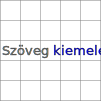
\includegraphics{images/concept/text.JPG}
    \end{adjustbox}
    \caption{Példa: Szöveges tartalom kódja és vizuális megjelenése}
    \label{fig:example_text}
\end{figure}


\subsubsection{Raszteres képek}

Az \lstinline[language=XML]|<image>| elem teszi lehetővé raszteres fájlok, például PNG vagy JPEG beágyazását a vektorgrafikus ábrába. Ez a mechanizmus hibrid tartalmak létrehozásához szükséges.

\begin{itemize}
    \item \texttt{x, y:} A kép bal felső sarkának koordinátái
    \item \texttt{width, height:} A kép megjelenítési mérete
    \item \texttt{href:} A képfájl forrásának URI-ja (elérési útja)
\end{itemize}

Az SVG szerkesztők a raszteres képeket általában \texttt{base64} formátumúvá alakítják. Majd ez a karakterlánc felhasznált a \texttt{href} attribútum értékeként.

\begin{figure}[!ht]
    \centering
    \begin{adjustbox}{valign=m, max width=0.8\textwidth}
        \begin{lstlisting}[language=XML]
    <image href="svg-logo.png"
        x="25" y="25" width="50" height="50" />
        \end{lstlisting}
    \end{adjustbox}
    \hfill
    \begin{adjustbox}{valign=m, max width=0.2\textwidth}
        \includesvg{images/concept/image.svg}
    \end{adjustbox}
    \caption{Példa: Kép kódja és vizuális megjelenése}
    \label{fig:example_img}
\end{figure}

\subsection{Prezentációs attribútumok}

Az SVG elemek geometriai meghatározása mellett a vizuális megjelenésüket a prezentációs attribútumok \cite{mdn-svg-attributes} határozzák meg. Ezek az attribútumok CSS tulajdonságként is értelmezhetők, így megadhatók közvetlenül az elemen attribútumként, vagy CSS stíluslapokon keresztül is.

\subsubsection{Körvonal}

A körvonal az alakzatok határvonalát jelenti. Az SVG szabvány számos attribútumot biztosít a vonalak végződésének, csatlakozásának és mintázatának beállítására.

\vspace{9pt}

\textbf{stroke:} A körvonal színét határozza meg. Értéke lehet konkrét színkód, színnév, vagy hivatkozás egy színátmenetre. Alapértelmezett értéke none, vagyis a körvonal nem látható.

\vspace{9pt}

\textbf{stroke-width:} A körvonal vastagságát definiálja. Értéke egy pozitív szám, amely az aktuális koordináta-rendszer egységében értendő, alapértéke az 1.

\vspace{9pt}

\textbf{stroke-opacity}: A körvonal átlátszóságát szabályozza 0.0 (teljesen átlátszó) és 1.0 (teljesen látható) között. Ez független az elem többi részének átlátszóságától.

\vspace{9pt}

\textbf{stroke-linecap}: Nyílt útvonalak végpontjainak alakját határozza meg. Három lehetséges értéke van:
\begin{itemize}
    \item \texttt{butt:} A vonal pontosan a végpontnál ér véget, levágott véggel. Ez az alapértelmezett érték.
    \item \texttt{round:} A vonal végét egy félkör zárja le, amelynek sugara a vonalvastagság fele.
    \item \texttt{square:} A vonal vége egy négyzetes lezárást kap, amely a vonalvastagság felével túlnyúlik a végponton.
\end{itemize}

\vspace{9pt}

\textbf{stroke-linejoin}: Két vonalszakasz találkozásánál, vagyis sarkánál kialakuló alakzat típusát adja meg. Három lehetséges értéke van:

\begin{itemize}
    \item \texttt{miter:} Hegyes sarok, ahol a külső élek a metszéspontig meghosszabbodnak. Ez az alapértelmezett érték.
    \item \texttt{round:} A sarok lekerekített.
    \item \texttt{square:} Levágott sarok, mintha egy egyenes vonallal összekötnénk a két szakasz külső pontjait.
\end{itemize}

\vspace{9pt}

\textbf{stroke-dasharray}: Szaggatott vonalak létrehozására szolgál. Értéke egy vesszővel vagy szóközzel elválasztott számsorozat, amely felváltva határozza meg a vonalszakaszok és a szünetek hosszát.

\subsubsection{Kitöltés}

A kitöltés az alakzatok belső területének színezését jelenti. Zárt alakzatoknál, mint például köröknél, egyértelmű a belső terület. Viszont nyílt útvonalaknál a végpontok összekötésével képzett területet jelöli.

\vspace{9pt}

\textbf{fill:} A belső terület színét határozza meg. Hasonlóan a stroke-hoz, lehet szín, átmenet vagy minta. Alapértelmezett értéke a fekete. A none érték használatával az alakzat belseje átlátszó marad.

\vspace{9pt}

\textbf{fill-opacity:} A kitöltés átlátszóságát állítja be, anélkül, hogy a körvonal átlátszóságát befolyásolná.

\vspace{9pt}

\textbf{fill-rule:} Önmagát metsző vagy lyukas útvonalak esetén határozza meg, hogy mely területek számítanak "belülnek" és melyek "kívülnek". Két főbb értéke van:

\begin{itemize}
    \item \texttt{nonzero:} Ez az alapértelmezett szabály. Egy adott pontból húzott sugár és az útvonal metszéspontjainak irányát vizsgálja. Ez lehet óramutató járásával megegyező vagy ellentétes. Ha az összeg nem nulla, a pont belül van.
    \item \texttt{evenodd:} Azt vizsgálja, hogy a sugár hányszor metszi az útvonalat. Ha a metszéspontok száma páratlan, a pont belül van. Ha ez a szám páros, akkor kívül van. Lehetővé teszi a lyukas alakzatok egyszerű létrehozását.
\end{itemize}

\subsubsection{Láthatóság}

Az \texttt{opacity} attribútum az elem átlátszóságát szabályozza. Értéke a 0.0 és 1.0 közötti tartományban mozoghat, ahol a nulla a teljes átlátszóságot, az egy pedig a teljes láthatóságot jelöli. Fontos különbség a kitöltési és körvonal átlátszósághoz képest, hogy csoportokra alkalmazva az attribútum a benne foglalt elemek összesített átlátszóságát határozza meg, így a megjelenítéskor az elemek egységesen halványodnak el, nem pedig egymáson áttűnve.

\subsubsection{Transzformációk}

A \texttt{transform} attribútum segítségével végezhető el az elemek geometriai manipulációja az eredeti koordináta-rendszerhez viszonyítva. A \texttt{translate(x, y)} parancs az eltolást végzi az x és y tengelyek mentén. A \texttt{rotate(a, x, y)} adott \texttt{a} szöggel és egy tetszőleges \texttt{x, y} középpont körül forgatja el az elemet. A \texttt{scale(x, y)} az elem átméretezését  teszi lehetővé az \texttt{x, y} tengelyeken. Egy paraméter használatával, tehát \texttt{scale(s)} esetén \texttt{s} mennyiséggel egységesen skálázza az elemet.

\subsubsection{Szűrők}
A \texttt{filter} attribútum használata komplex vizuális effektek, például elmosás, árnyékvetés vagy színkorrekció alkalmazását teszi lehetővé. Az attribútum értéke jellemzően a definíciós szekcióban létrehozott szűrőelem egyedi azonosítójára hivatkozik, amelyet az URL szintaxis segítségével kapcsolunk a grafikus elemhez.

\subsubsection{Vágás}
A \texttt{clip-path} egy specifikus SVG mechanizmus, amely a látható terület korlátozására szolgál. Egy másik SVG alakzat, például egy kör vagy vonal segítségével vágja le a megjelenítendő elemet. A definiált vágási területen kívül eső részek a megjelenítéskor nem láthatók.

\subsubsection{Maszkolás}
A maszkolás a vágáshoz hasonló technika, azonban itt a maszkoláshoz használt elem szürkeárnyalatos értékei határozzák meg az átlátszóság mértékét. A \texttt{mask} attribútummal használható. A fehér szín a teljes láthatóságot, a fekete a teljes átlátszóságot, a köztes szürke árnyalatok pedig félig áttetsző megjelenést eredményez.

\subsection{Csoportosítás és struktúra}

Az SVG dokumentumok egyik legfontosabb szervezőeleme a \lstinline[language=XML]|<g>| (group) tárolóelem, amely logikailag és strukturálisan összefogja a benne elhelyezett objektumokat. Használata lehetővé teszi az összetartozó komponensek, például egy ikon részleteinek egyetlen egységként való kezelését. A csoportosítás befolyásolja a transzformációkat is. Az eltolás, forgatás vagy skálázás egységesen érvényesülnek minden a csoportban lévő elemre. Hasonlóan működik a megjelenési attribútumok esetén, a kitöltés vagy a körvonal stílusa automatikusan öröklődnek. Kivéve, ha azok saját beállítással felülírják azt.

Az alábbi példában a csoport fekete körvonalat és egy eltolást definiál. A kör örökli a fekete körvonal színt, míg a téglalap felülírja azt saját kék színével, de az eltolás mindkettőre vonatkozik.

\begin{figure}[!ht] \centering
    \begin{adjustbox}{valign=m, max width=0.8\textwidth} 
        \begin{lstlisting}[language=XML]
        <g transform="translate(10,10)"
            stroke="black" stroke-width="2" fill="none">
            <circle cx="30" cy="30" r="15" />
            <rect x="55" y="15" width="30" height="30" stroke="blue" />
        </g>
        \end{lstlisting}
    \end{adjustbox}
    \hfill
    \begin{adjustbox}{valign=m, max width=0.2\textwidth}
        \includesvg{images/concept/group.svg}
    \end{adjustbox}
    \caption{Példa: Csoportosítás, transzformáció és stílusöröklés hatása, kód és megjelenés}
    \label{fig:example_group}
\end{figure}

\section{Szerkesztőeszközök}

Több SVG szerkesztő is elérhető, amelyek különböző célközönségeknek megfelelő funkcionalitást kínálnak. Egyes esetekben nagyon bő a funkcionalitások választéka, ami magas tanulási görbét eredményezhet. Más esetekben számos előre definiált alakzat áll rendelkezésre, viszont korlátozottak a grafikus szerkesztő eszközök. Az alábbiakban megismerkedhetünk néhány népszerű asztali és webes SVG szerkesztő alkalmazással. Kifejtésre kerülnek összehasonlító szempontok, amik kritériumok lesznek a saját szerkesztőm felé.

\subsection{Boxy SVG}

\begin{figure}[H]
\centering
\includegraphics[width=0.8\textwidth]{images/concept/boxy-svg-interface.JPG}
\caption{A Boxy SVG kezelőfelülete \cite{boxy-svg}}
\label{fig:boxy-svg}
\end{figure}

A Boxy SVG (\ref{fig:boxy-svg}. ábra) egy vektorgrafikus szerkesztő, amely elérhető webalkalmazásként és asztali alkalmazásként is. A szerkesztőfelület fejlécében egy menüsor van, amellyel elérhető a szerkesztő összes funkcionalitása. Alatta egy transzformációs sáv, amely gyors elérést ad alap csoportosítási, igazítási, forgatási és Boolean operációs eszközökhöz. Középen a rajzoló vászon jelenik meg, ezt körbevéve az úgynevezett vonalzók. Ezek pixelben mérve jelölik a vászon méretét, a kijelölt objektumok méretét és a kurzor pozicíját.

Az SVG szabványban definiált alapelemeken túl ad lehetőséget gyakran használt alakzatok, mint háromszög vagy csillag rajzolására. Ezek beállításai egy bal oldali lebegő ablakban jelenik meg. A tulajdoságok a jobb oldali sávból érhetők el, egy kattintásra beúszó ablakban állíthatók be. Az alsó két gombbal elérhető a kódszerkesztő és az animációs panel, amik alulról úsznak be. A kódszerkesztőben módosítható az SVG egész forráskódja és az adott elem stílusozása is, a változtatás azonnal megjelenik.

Teljeskörű szövegszerkesztésre ad lehetőséget, a legtöbb általános szöveg beállítás megadható. A szöveg in-place, tehát egyenesen a vásznon szerkeszthető. A színek és stílusok megadása széleskörű. Támogatja a lineáris és radiális gradiensek, valamint mintázatok létrehozását. A felhasználó előre definiált színkönyvtárakat is használhat. Az útvonalszerkesztés a szerkesztőeszközzel valósul meg, a csomópontoknál Bézier-fogantyúkkal manipulálható. Támogatja az unió, kivonás, metszet és komplementer logikai műveleteket az alakzatok között.

Az elrendezést segédvonalak és rácshoz igazítás segíti, amely jelzi az objektumok egymáshoz viszonyított helyzetét. Van lehetőség külön réteg és csoport kezelésre, fa struktúrában látható a DOM hierarchia. Az elemek sorrendje drag-and-drop módszerrel módosítható. A kijelölés történhet kattintással vagy terület kijelöléssel, támogatva a csoportos műveleteket is. A rendszerszintű vágólap műveletek, mint a másolás és beillesztés, billentyűkombinációkkal is elérhetők. A nagyítás és navigáció az egérgörgővel és gesztusokkal intuitív módon működik. A visszavonási előzmények mélyrehatóak, számos lépés visszakereshető. A mentés automatikusan történik a felhőbe.

\subsection{SVG-Edit}

\begin{figure}[H]
\centering
\includegraphics[width=0.8\textwidth]{images/concept/svg-edit-interface.JPG}
\caption{Az SVG-Edit kezelőfelülete \cite{svg-edit}}
\label{fig:svg-edit}
\end{figure}

Az SVG-Edit (\ref{fig:svg-edit}. ábra) egy nyílt forráskódú, webalapú szerkesztő. A szerkesztő fejlécében lévő menüsor a fájl kezelésére, nézet beállítására és transzformációk beállítására szolgál.

Bal oldalon helyezkedik el az eszköztár kijelölő és rajzoló eszközökkel. Az alapelemek közül támogatja a szabványos alakzatokat, valamint rendelkezik egy beépített alakzat könyvtárral. A kiválasztott objektumok tulajdonságai, mint a kitöltés vagy körvonal, az alsó sávban módosíthatók. Egy dedikált gombbal megnyitható az SVG kódablak, ahol az XML szöveg szerkeszthető. A módosítások elfogadása után jelennek meg a változtatások a vásznon.

A szövegszerkesztés a vásznon történik, elég részletesen szabályozható a karakterek beállítása. Viszont nem támogatja a többsoros bevitelt és csak hét alap betűtípust biztosít. A színeket alap RGBA és HSV értékekkel van lehetőség megadni a bal alsó színválasztóban. Beállítható a színezés típusa is, lehet egyszínű, lineáris színátmenet vagy radiális színátmenet. Az útvonalszerkesztő eszköz lehetővé teszi a csomópontok mozgatását és törlését, de a Bézier-fogantyúk kezelése nem teljesen intuitív. Az igazításhoz bekacsolható rácsháló, egyénileg és csoportosan is rendezhetők objektumok. A rétegkezelés a jobb panelen érhető el, ahol az elemek sorrendje és láthatósága állítható. Támogatja a rendszerszintű másolás-beillesztés műveleteket, valamint rendelkezik előzmény kezeléssel is. Az automatikus mentés beállítható, alapvetően a böngésző helyi tárolójába történik.

\subsection{Inkscape}

\begin{figure}[H]
\centering
\includegraphics[width=0.8\textwidth]{images/concept/inkscape-interface.JPG}
\caption{Az Inkscape kezelőfelülete \cite{inkscape}}
\label{fig:inkscape}
\end{figure}

Az Inkscape (\ref{fig:inkscape}. ábra) egy professzionális, nyílt forráskódú asztali vektorgrafikus szerkesztő. Felülete rendkívül összetett, bal oldalon a részletes eszköztár, felül az eszközvezérlő sáv és a menüsor, jobb oldalon dokkolható párbeszédablakok, alul pedig a színpaletta és az állapotsor található.

Az alapelemek létrehozása mellett számos speciális alakzatot is támogat. A tulajdonságok numerikus beállítását dedikált panelek teszik lehetővé. A beépített XML szerkesztő fa-struktúrában jeleníti meg a DOM-ot, lehetőséget adva bármely attribútum valós idejű módosítására. A kód nemcsak olvasható, hanem teljes mértékben írható is, a változások megerősítés után érvényesülnek.

A szövegszerkesztés nagyon részletes, támogatja a betűközök, sorközök és szöveg folyatását görbére illesztve. Dedikált szöveg szerkesztő ablak is tartozik hozzá, ha nem in-place szövegszerkesztést szeretnénk szöveget szerkeszteni. Színkezelése teljes körű, beleértve a CMYK, HSL és RGB színtereket, valamint a komplex gradienseket és mintázatokat. Az útvonalszerkesztés a szoftver egyik legnagyobb erőssége. A csomópont eszköz teljes testreszabhatóságot ad a Bézier-görbék felett. Támogatja a csomópontok típusának váltását és a logikai műveleteket. A rétegkezelés hierarchikus, van opció csoportosításra és rétegek zárolására. Rendelkezik automatikus mentési és helyreállítási funkcióval is.

\subsection{Figma}

\begin{figure}[H]
\centering
\includegraphics[width=0.8\textwidth]{images/concept/figma-interface.JPG}
\caption{A Figma kezelőfelülete \cite{figma}}
\label{fig:figma}
\end{figure}

A Figma (\ref{fig:figma}. ábra) egy felülettervező eszköz, amely bár elsődlegesen UI/UX designra készült, erős vektorgrafikus képességekkel rendelkezik. Elrendezése minimalista, a bal oldali sáv a rétegeket és az eszközöket, a jobb oldali sáv a tulajdonságokat tartalmazza, míg a középső vászon a munkafelület.

Az alapelemek egy legördülő menüből érhetők el, de nem túl bőséges a választék. A tulajdonságok szerkesztése a jobb oldali panelen történik, ahol az értékek gombokkal, csúszkákkal vagy numerikusan is megadhatók. Bár az SVG importálása és exportálása megbízhatóan működik, a felhasználó nem szerkesztheti közvetlenül az SVG struktúrát.

A szövegkezelés fejlett, támogatja a Google Fonts integrációt és a részletes tipográfiai beállításokat. A színkezelés stílus könyvtárakra épül, lehetővé téve a színek globális definiálását és újrafelhasználását. Az útvonalszerkesztést a Figma egyedi módon kezeli, a "Vector Networks" technológiával. Ez lehetővé teszi, hogy egy csomópontból kettőnél több vonal induljon ki, egyszerűbbé téve a rajzolást. Az igazítási funkciók és az automatikus elrendezés részletesek. A rétegkezelés fa-struktúrában történik, támogatva a mély kijelölést (Ctrl+Click). A mentés folyamatos és automatikus a felhőbe, teljes verziótörténettel rendelkezik.

\subsection{Mediamodifier}

\begin{figure}[H]
\centering
\includegraphics[width=0.8\textwidth]{images/concept/mediamodifier-interface.JPG}
\caption{A Mediamodifier kezelőfelülete \cite{mediamodifier}}
\label{fig:mediamodifier}
\end{figure}

A Mediamodifier (\ref{fig:mediamodifier}. ábra) egy online marketingeszköz, amely a sablonok testreszabására és mockupok készítésére fókuszál. A felület egyszerűsített webes elrendezést követ. Bal oldalon található egy alapvető eszköz sáv, jobb oldalon a tulajdonság beállító panel, középen pedig a vászon.

A szoftver nem a rajzolásra, hanem a kész elemek összeállítására helyezi a hangsúlyt. Tartalmaz alapvető alakzatokat, de ezek inkább matricaként működnek. A tulajdonságok szerkesztése korlátozott. A jobb oldali sávban csúszkákkal állítható az átlátszóság és körvonal méret. A forráskódhoz való hozzáférés teljes mértékben hiányzik, a felhasználó nem látja és nem módosíthatja az SVG struktúrát.

A szövegszerkesztés in-place módon történik, de a formázási lehetőségek kimerülnek a betűtípus és szín választásában. A színkezelés egyszerű színválasztókkal működnek, az átlátszósághoz külön csúszka tartozik és HEX kódként kezeltek. Nincs lehetőség görbéket rajzolni és nincs útvonalszerkesztés. A rétegkezelés csupán az elemek sorrendjének előre vagy hátra állítását teszi lehetővé. A mentés manuális vagy fiókhoz kötött.

\subsection{Összehasonlítás}

Az összehasonlítást az alábbi szempontok alapján végzem el:

\begin{description}

\item[Elrendezés:] Az elrendezés határozza meg a felhasználó első benyomását. Fontos, hogy a felület átlátható legyen, és a gyakori eszközök kézre essenek. Két fő irányvonal figyelhető meg:

\begin{itemize}
    \item \textit{Klasszikus:} Bal oldali eszköztár, felső menüsor és jobb oldali tulajdonság panelek. Néhány felugró ablak vagy panel.
    \item \textit{Panelek és lebegő elemek:} Lebegő panelek, alapvető eszköz sávok, ahol a vászon kapja a legnagyobb teret.
\end{itemize}

\item[Alapelemek megjelenítése:] Az SVG szabványban definiált alapelemek elérésének módja. A felhasználó szempontjából előnyös, ha ezek logikusan csoportosítva jelennek meg, és nem ömlesztve. Szempont továbbá, hogy támogat-e a szerkesztő komplexebb, előre definiált alakzatokat.

\item[Tulajdonságok szerkesztése:] A már létrehozott objektumok utólagos módosíthatósága a grafikus felületen keresztül. Ez magában foglalja a transzformációkat és a vizuális attribútumokat. Fontos szempont, hogy a vizuális manipuláció mellett ezek az értékek numerikusan is megadhatók legyenek.

\item[Kód nézet és szerkesztés:] A grafikus szerkesztők egyik legfontosabb pontja fejlesztői szempontból. Azt vizsgálom, hogy a felhasználó hozzáfér-e a generált SVG forráskódhoz szerkesztés közben:
\begin{itemize}
    \item \textit{Élő szerkesztés:} A kódpanelen végzett módosítás megerősítés után vagy azonnal megjelenik a vásznon. Ezek külön kategorizáltak XML, forrás és konkrét szerkesztő nézetre.
    \item \textit{Nincs:} A szerkesztő teljesen elrejti a forráskódot.
\end{itemize}

\item[Szövegek szerkesztése:] Van-e lehetőség több soros, bekezdésés szöveg beszúrására, vagy csak egy sorba kerül. A szerkesztőnek biztosítania kell a betűtípus, méret, stílus és igazítás beállításait. A szöveg szerkesztése közvetlenül a vásznon \textit{"in-place"} történik-e. Alternatívan egy felugró ablakban vagy külön beviteli mezőben.

\item[Színek és stílusok megadása:] Az SVG stílusozás és CSS kezelése.
\begin{itemize}
    \item A kitöltés és körvonal támogatja-e az RGB, HEX, HSL színmegadást, valamint az átlátszóságot.
    \item Van-e lehetőség lineáris és radiális színátmenetek, illetve mintázatok létrehozására és szerkesztésére.
\end{itemize}

\item[Útvonalszerkesztés:] Milyen szinten támogatott a \lstinline[language=XML]|<path>| elem manipulációja. A szempont azt vizsgálja, hogyan kezelhetők a csomópontok:
\begin{itemize}
    \item Hozzáadhatók és törölhetők-e pontok?
    \item A Bézier-görbék kontrollpontjai, fogantyúi intuitívan mozgathatók-e?
    \item Támogatja-e a logikai műveleteket, mint unió, különbség, metszet és komplementer az alakzatok között.
\end{itemize}

\item[Objektumok automatikus igazítása:] Rendelkezik-e a szerkesztő "mágneses" funkcióval, amely az objektumokat rácspontokhoz, más objektumok éleihez vagy középpontjához igazítja mozgatás közben.

\item[Rétegek és csoportok kezelése:] Az SVG DOM struktúrájának kezelése. Van-e lehetőség elemek csoportosítására, illetve külön rétegek létrehozására. Fontos, hogy a szerkesztő vizuálisan megjelenítse a hierarchiát, és lehetővé tegye az elemek sorrendjének drag-and-drop módosítását.

\item[Kijelölés:] Milyen módszerekkel választhatók ki az elemek. Kattintással kiválasztható egy elem, téglalap alapú kijelöléssel több is. \textit{Shift} vagy \textit{Ctrl} billentyűkkel több elem együttes kezelése.

\item[Másolás és beillesztés:] Működnek-e a rendszerszintű vágólap műveletek. A másolás \texttt{Ctrl+C}, a beillesztés \texttt{Ctrl+V} és a vágás \texttt{Ctrl+X} billenytűkombinációkkal. Webes környezetben ez biztonsági korlátok miatt gyakran nehézkes, ezért vizsgálom, hogy van-e belső megoldás az elemek duplikálására.

\item[Nagyítás:] Mivel az SVG skálázható, a vászon nagyításának és mozgatásának intuitívnak kell lennie. Egérgörgővel vagy gesztusokkal is vizsgáltam a funkcionalitás működését.

\item[Undo-Redo funkciók:] Az előzmények kezelése. Van-e lehetőség a műveletek visszavonására és megismétlésére. Ez mennyire mélyreható, hány lépést jegyez meg a rendszer. Elvárás a visszavonás \texttt{Ctrl+Z}, és megismétlés \texttt{Ctrl+Y / Shift+Z} billentyűkombinációk támogatása.

\item[Automatikus mentés:] Webes alkalmazásoknál kritikus, hogy hálózati hiba vagy véletlen bezárás esetén megmarad-e a munka. A szerkesztő menti-e a böngésző helyi tárolójába (Local Storage) vagy felhőbe az állapotot.
\end{description}

\noindent Ezeket az összehasonlítási szempontokat tartalmazza a \ref{tab:svg-editors-comparison}. táblázat.

\begin{table}[ht]
\caption{Webes és asztali SVG szerkesztők funkcionális összehasonlítása}
\label{tab:svg-editors-comparison}
\medspace
\centering
\footnotesize
\begin{adjustbox}{max width=\textwidth}
\begin{tabular}{|l|c|c|c|c|c|c|}
\hline
 & \textbf{Inkscape} & \textbf{SVG-Edit} & \textbf{Boxy SVG} & \textbf{Figma} & \textbf{MediaM.} \\ \hline

\textbf{Elrendezés} & 
\multicolumn{3}{c|}{Klasszikus} & 
\multicolumn{2}{c|}{Panelek / Lebegő elemek} \\ \hline

\textbf{Alapelemek} & 
\multicolumn{5}{c|}{Bal oldali sáv} \\ \hline

\textbf{\begin{tabular}[c]{@{}l@{}}Tulajdonság\\ szerk.\end{tabular}} & 
\begin{tabular}[c]{@{}c@{}@{}}Felső és\\ Alsó sáv +\\ Jobb panel\end{tabular} & 
\begin{tabular}[c]{@{}c@{}}Felső +\\ Alsó sáv\end{tabular} & 
\begin{tabular}[c]{@{}c@{}}Felső sáv +\\ Jobb panel\end{tabular} & 
\multicolumn{2}{c|}{\begin{tabular}[c]{@{}c@{}}Jobb \\ panel\end{tabular}} \\ \hline

\textbf{Kód nézet} & 
\begin{tabular}[c]{@{}c@{}}Élő\\ XML\end{tabular} & 
\begin{tabular}[c]{@{}c@{}}Élő\\ Forrás\end{tabular} & 
\begin{tabular}[c]{@{}c@{}}Élő\\ Szerkesztő\end{tabular} & 
\multicolumn{2}{c|}{Nincs} \\ \hline

\textbf{Szöveg} & 
\begin{tabular}[c]{@{}c@{}}In-place +\\ szerkesztő\end{tabular} & 
\multicolumn{4}{c|}{In-place} \\ \hline

\textbf{Színek} & 
Teljes & 
\begin{tabular}[c]{@{}c@{}}RGBA\\ HSV\end{tabular} & 
\multicolumn{2}{c|}{\begin{tabular}[c]{@{}c@{}}Könyvtárak,\\ Gradiensek\end{tabular}} &
\begin{tabular}[c]{@{}c@{}}HEX\\ kód\end{tabular} \\ \hline

\textbf{\begin{tabular}[c]{@{}l@{}}Útvonal-\\ szerkesztés\end{tabular}} & 
\begin{tabular}[c]{@{}c@{}}Teljes\\ körű\end{tabular} & 
Alapvető & 
Fejlett &
\begin{tabular}[c]{@{}c@{}}Vector\\ networks\end{tabular} &
Nincs \\ \hline

\textbf{Igazítás} & 
Fejlett & 
Alap & 
\multicolumn{2}{c|}{\begin{tabular}[c]{@{}c@{}}Okos\\ segédvonalak\end{tabular}} & 
Alap \\ \hline

\textbf{Rétegek} & 
\multicolumn{4}{c|}{Teljes hierarchia kezelés} & 
\begin{tabular}[c]{@{}c@{}}Előre-hátra\\ tolás\end{tabular} \\ \hline

\textbf{Kijelölés} & 
\multicolumn{4}{c|}{Terület + Kattintás + Csoportos} & 
\begin{tabular}[c]{@{}c@{}}Terület +\\ Kattintás\end{tabular} \\ \hline

\textbf{\begin{tabular}[c]{@{}l@{}}Másolás és\\ beillesztés\end{tabular}} & 
\multicolumn{5}{c|}{Gombok és billenytűkombinációk} \\ \hline

\textbf{Nagyítás} &
\begin{tabular}[c]{@{}c@{}}Gombok és\\ billenytűk.\end{tabular} & 
\begin{tabular}[c]{@{}c@{}}Opciók és\\ gombok\end{tabular} & 
\multicolumn{3}{c|}{Gombok és billenytűkombinációk} \\ \hline

\textbf{\begin{tabular}[c]{@{}l@{}}Automatikus\\ mentés\end{tabular}} & 
Igen & 
Helyi tároló & 
\multicolumn{2}{c|}{Felhő alapú} & 
Nem \\ \hline

\end{tabular}
\end{adjustbox}
\end{table}